\graphicspath{{chapter_faces/}}
\chapter{Large Pose 3D Face Reconstruction via Volumetric Regression}
\label{chapter:face}

\begin{figure}
  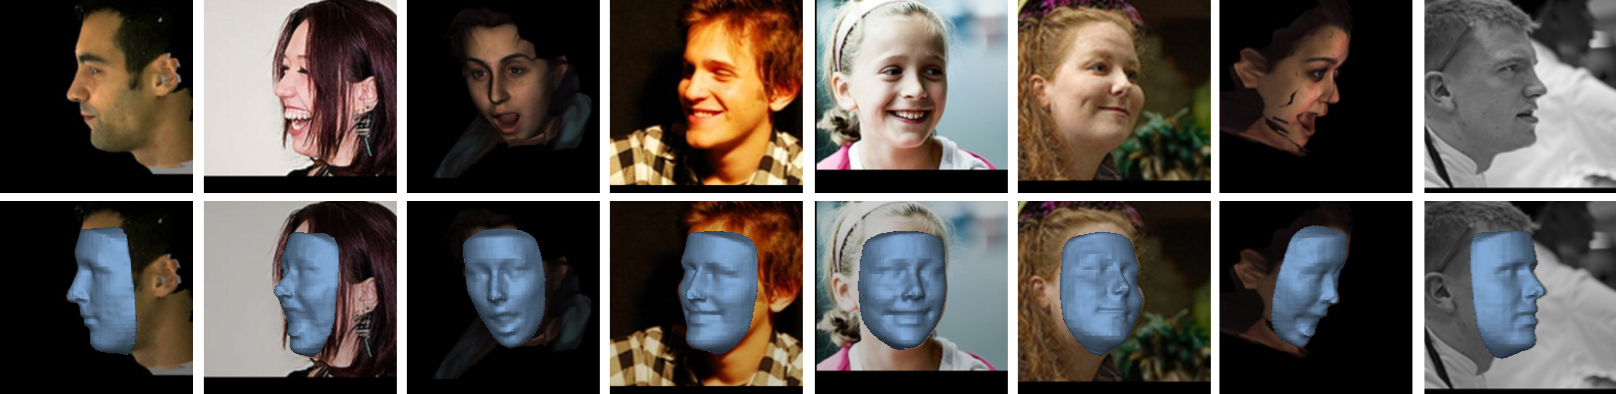
\includegraphics[width=\linewidth]{img/preview.png}
  \caption[A 3D Reconstruction Preview]{A preview of our 3D
    reconstruction method, applied on a wide variety of poses.}
  \label{c:face:fig:preview}
\end{figure}
% \begin{abstract}
%   3D face reconstruction is a fundamental Computer Vision problem of
%   extraordinary difficulty. Current systems often assume the
%   availability of multiple facial images (sometimes from the same
%   subject) as input, and must address a number of methodological
%   challenges such as establishing dense correspondences across large
%   facial poses, expressions, and non-uniform illumination. In general
%   these methods require complex and inefficient pipelines for model
%   building and fitting. In this work, we propose to address many of
%   these limitations by training a Convolutional Neural Network (CNN)
%   on an appropriate dataset consisting of 2D images and 3D facial
%   models or scans. Our CNN works with just a single 2D facial image,
%   does not require accurate alignment nor establishes dense
%   correspondence between images, works for arbitrary facial poses and
%   expressions, and can be used to reconstruct the whole 3D facial
%   geometry (including the non-visible parts of the face) bypassing the
%   construction (during training) and fitting (during testing) of a 3D
%   Morphable Model. We achieve this via a simple CNN architecture that
%   performs direct regression of a volumetric representation of the 3D
%   facial geometry from a single 2D image. We also demonstrate how the
%   related task of facial landmark localization can be incorporated
%   into the proposed framework and help improve reconstruction quality,
%   especially for the cases of large poses and facial
%   expressions. Code and models will be made available at \verb|http://aaronsplace.co.uk|
% \end{abstract}
% \vspace{-4mm}

3D face reconstruction is a fundamental Computer Vision problem, often
considered to be of extraordinary difficultly. Current systems often
assume the availability of multiple facial images as input, sometimes
from the same subject. Additional, there are a number of
methodological challenges involved, which must be addressed. These
challenges include establishing a dense correspondence across large
poses, expressions and non-uniform illumination. In general, these
methods require complex and inefficient pipelines for model building
and fitting. IN this work, we propose to address many of these
limitations by constraining the problem of 3D face reconstruction to
the spatial domain. We do this by training a Convolutional Neural
Network (CNN), on an appropriate dataset, consisting of 2D images and
3D facial models, or scans. Our CNN works with just a single 2D facial
image and does not require accurate alignment. Our method works for
arbitrary facial poses and expressions, and can be used to
reconstruction the whole 3D facial geometry, including non-visible
parts. Our method bypasses the construction (during training) and
fitting (during inference) of a 3D Morphable Model. We achieve this via
a simple CNN architecture that performs direct regression of a
volumetric representation of the 3D facial geometry from a single 2D
image. We also demonstrate how the related task of facial landmark
localisation can be incorporated into the proposed framework and help
improve reconstruction quality, especially in the cases of large poses
and facial expressions.


\section{Introduction}
3D face reconstruction is the problem of recovering the 3D facial
geometry from 2D images. Despite many years of research, it is still
an open problem in Vision and Graphics research. Depending on the
setting and the assumptions made, there are many variations of it as
well as a multitude of approaches to solve it. This work is on 3D face
reconstruction using only a single image. Under this setting, the
problem is considered far from being solved. In this chapter, we
propose to approach it, for the first time to the best of our
knowledge, by directly learning a mapping from pixels to 3D
coordinates using a Convolutional Neural Network (CNN). Besides its
simplicity, our approach works with totally unconstrained images
downloaded from the web, including facial images of arbitrary poses,
facial expressions and occlusions, as shown in
Figure~\ref{c:face:fig:preview}. \newline \textbf{Motivation.} No matter what
the underlying assumptions are, what the input(s) and output(s) to the
algorithm are, 3D face reconstruction requires in general complex
pipelines and solving non-convex difficult optimization problems for
both model building (during training) and model fitting (during
testing). In the following paragraph, we provide examples from 5
predominant approaches:

\begin{enumerate}
\item In the 3D Morphable Model (3DMM) \cite{blanz1999morphable,
    romdhani2005estimating}, the most popular approach for estimating
  the full 3D facial structure from a single image (among others),
  training includes an iterative flow procedure for dense image
  correspondence which is prone to failure. Additionally, testing requires a
  careful initialisation for solving a difficult highly non-convex
  optimization problem, which is slow.
\item The work of \cite{kemelmacher20113d}, a popular approach for
  2.5D reconstruction from a single image, formulates and solves a
  carefully initialised (for frontal images only) non-convex
  optimization problem for recovering the lighting, depth, and albedo
  in an alternating manner where each of the sub-problems is a
  difficult optimization problem per se.
\item In \cite{kemelmacher2011face}, a quite popular recent approach
  for creating a neutral subject-specific 2.5D model from a near
  frontal image, an iterative procedure is proposed which entails
  localising facial landmarks, face frontalization, solving a
  photometric stereo problem, local surface normal estimation, and
  finally shape integration.
\item In \cite{suwajanakorn2014total}, a state-of-the-art pipeline for
  reconstructing a highly detailed 2.5D facial shape for each video
  frame, an average shape and an illumination subspace for the
  specific person is firstly computed (offline), while testing is an
  iterative process requiring a sophisticated pose estimation
  algorithm, 3D flow computation between the model and the video
  frame, and finally shape refinement by solving a shape-from-shading
  optimization problem.
\item More recently, the state-of-the-art method of
  \cite{roth2016adaptive} that produces the average (neutral) 3D face
  from a collection of personal photos, firstly performs landmark
  detection, then fits a 3DMM using a sparse set of points, then
  solves an optimization problem similar to the one in
  \cite{kemelmacher2011face}, then performs surface normal estimation
  as in \cite{kemelmacher2011face} and finally performs surface
  reconstruction by solving another energy minimisation problem.
\end{enumerate}

Simplifying the technical challenges involved in the aforementioned
works is the main motivation of this work.

\subsection{Main contributions}
We describe a very simple approach which bypasses many of the
difficulties encountered in 3D face reconstruction by using a
novel volumetric representation of the 3D facial geometry, and
an appropriate CNN architecture that is trained to regress directly
from a 2D facial image to the corresponding 3D volume. An overview of
our method is shown in Figure~\ref{fig:cnnall}. In summary, our contributions
are:
\begin{itemize}
\item Given a dataset consisting of 2D images and 3D face scans, we
  investigate whether a CNN can learn directly, in an end-to-end
  fashion, the mapping from image pixels to the full 3D facial
  structure geometry (including the non-visible facial parts). Indeed,
  we show that the answer to this question is positive.
\item We demonstrate that our CNN works with just a single 2D facial
  image, does not require accurate alignment nor establishes dense
  correspondence between images, works for arbitrary facial poses and
  expressions, and can be used to reconstruct the whole 3D facial
  geometry bypassing the construction (during training) and fitting
  (during testing) of a 3DMM.
\item We achieve this via a simple CNN architecture that performs
  \textit{direct} regression of a volumetric representation of the 3D
  facial geometry from a single 2D image. 3DMM fitting is not
  used. Our method uses only 2D images as input to the proposed CNN
  architecture.
\item We show how the related task of 3D facial landmark localisation
  can be incorporated into the proposed framework and help improve
  reconstruction quality, especially for the cases of large poses and
  facial expressions.
\item We report results for a large number of experiments on both
  controlled and completely unconstrained images from the web,
  illustrating that our method outperforms prior work on single image
  3D face reconstruction by a large margin.
\end{itemize}

\section{Method}


This section describes our framework including the proposed data representation used.


\subsection{Dataset}

Our aim is to regress the full 3D facial structure from a 2D image. To
this end, our method requires an appropriate dataset consisting of 2D
images and 3D facial scans. As our target is to apply the method on
completely unconstrained images from the web, we chose the dataset of
\cite{zhu2016face} for forming our training and test sets. The dataset
has been produced by fitting a 3DMM built from the combination of the
Basel \cite{paysan20093d} and FaceWarehouse
\cite{cao2014facewarehouse} models to the unconstrained images of the
300W dataset \cite{sagonas2013semi} using the multi-feature fitting
approach of \cite{romdhani2005estimating}, careful initialisation and
by constraining the solution using a sparse set of landmarks. Face
profiling is then used to render each image to 10-15 different poses
resulting in a large scale dataset (more than 60,000 2D facial images
and 3D meshes) called 300W-LP. Note that because each mesh is
produced by a 3DMM, the vertices of all produced meshes are in dense
correspondence; however this is not a prerequisite for our method and
unregistered raw facial scans could be also used if available
(e.g. the BU-4DFE dataset~\cite{yin2008high}).

\subsection{Proposed volumetric representation}

Our goal is to predict the coordinates of the 3D vertices of each
facial scan from the corresponding 2D image via CNN regression. As a
number of works have pointed out (see for example
\cite{tompson2015efficient, pfister2015flowing}), direct regression of
all 3D points concatenated as a vector using the standard L2 loss
might cause difficulties in learning because a single correct value
for each 3D vertex must be predicted. Additionally, such an approach
requires interpolating all scans to a vector of a fixed dimension, a
pre-processing step not required by our method. Note that similar
learning problems are encountered when a CNN is used to regress model
parameters like the 3DMM parameters rather than the actual
vertices. In this case, special care must be taken to weight
parameters appropriately using the Mahalanobis distance or in general
some normalisation method, see for example \cite{zhu2016face}. We
compare the performance of our method with that of a similar
method~\cite{zhu2016face} in Section~\ref{S:Results}.

\begin{figure}
  \centering
  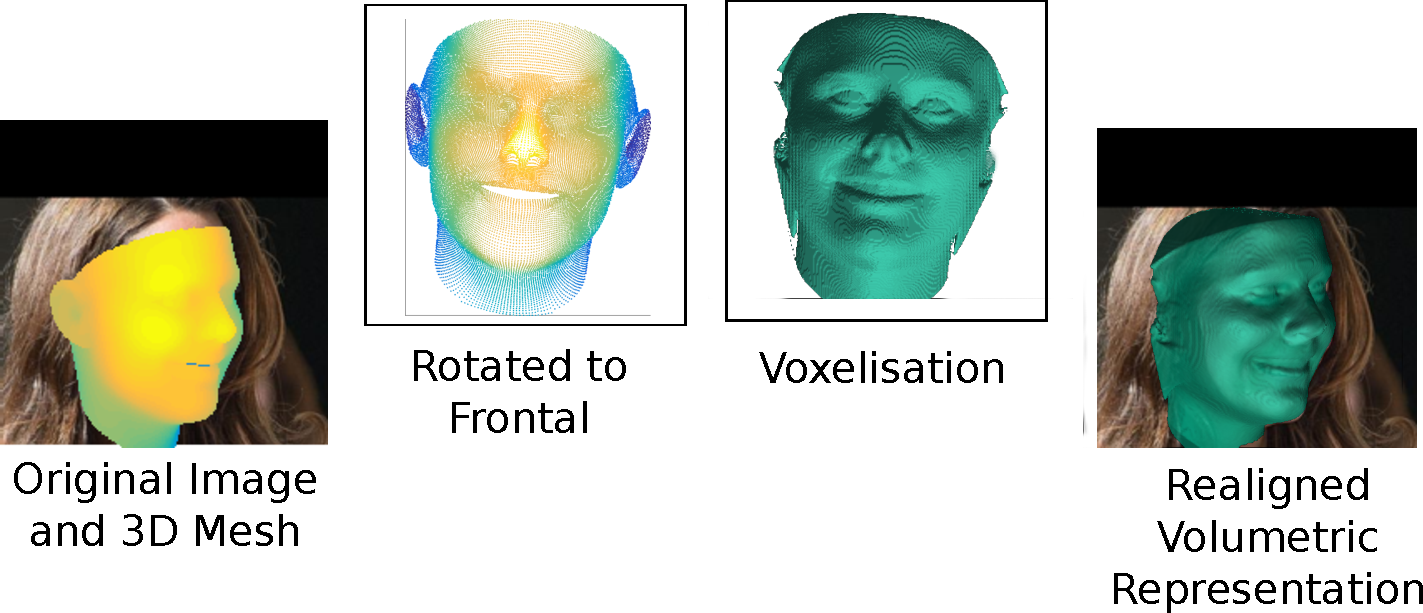
\includegraphics[width=0.7\linewidth]{img/discretisation.pdf}
  \caption[Dataset voxelisation procedure]{The voxelisation process
    creates a volumetric representation of the 3D face mesh, aligned
    with the 2D image.}
  \label{fig:discretisation}
\end{figure}

% Is it reasonable to say 2D to 3D image segmentation?
To alleviate the aforementioned learning problem, we propose to
reformulate the problem of 3D face reconstruction as one of 2D to 3D
image segmentation: in particular, we convert each 3D facial scan into
a 3D binary volume $\mathbf{V}_{whd}$ by discretizing the 3D space
into voxels $\{w,h,d\}$, assigning a value of 1 to all points enclosed
by the 3D facial scan, and 0 otherwise. That is to say $ V_{whd}$ is
the ground truth for voxel $\{w,h,d\}$ and is equal to 1, if voxel
$\{w,h,d\}$ belongs to the 3D volumetric representation of the face
and 0 otherwise (i.e. it belongs to the background). The conversion is
shown in Figure~\ref{fig:discretisation}. Notice that the process
creates a volume fully aligned with the 2D image. The importance of
spatial alignment is analysed in more detail in
Section~\ref{sec:spatialimportance}. The error caused by
discretization for a randomly picked facial scan as a function of the
volume size is shown in Figure~\ref{fig:voxerror}. Given that the error
of state-of-the-art methods \cite{roth2016adaptive,liu2016joint} is of
the order of a few mms, we conclude that discretization by
$192\times 192\times 200$ produces negligible error.

Given our volumetric facial representation, the problem of regressing
the 3D coordinates of all vertices of a facial scan is reduced to one
of 3D binary volume segmentation. We approach this problem using
recent CNN architectures from semantic image segmentation
\cite{long2015fully} and their extensions \cite{newell2016stacked}, as
described in the next subsection.

\begin{figure}
  \centering
  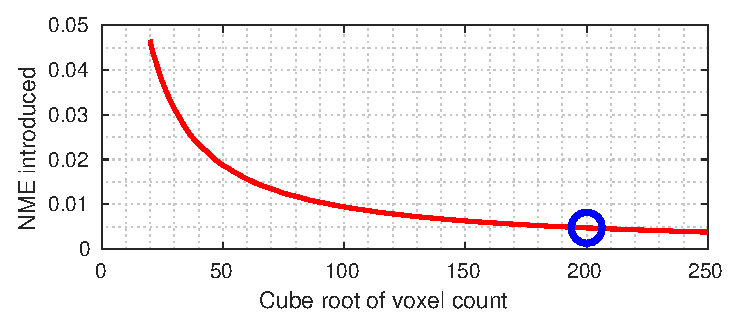
\includegraphics[width=0.75\linewidth]{curves/voxerror.eps}
  \caption[Error due to voxelisation]{The error introduced due to
    voxelisation, shown as a function of volume density.}
  \label{fig:voxerror}
\end{figure}

\subsection{Volumetric Regression Networks}


In this section, we describe the proposed volumetric regression
network, exploring several architectural variations described in
detail in the following subsections:

\textbf{Volumetric Regression Network (VRN)}. We wish to learn a
mapping from the 2D facial image to its corresponding 3D volume
$f: \mathbf{I} \rightarrow \mathbf{V}$. Given the training set of 2D
images and constructed volumes, we learn this mapping using a CNN. Our
CNN architecture for 3D segmentation is based on the ``hourglass
network'' of \cite{newell2016stacked} an extension of the fully
convolutional network of \cite{long2015fully} using skip connections
and residual learning \cite{he2015deep}. Our volumetric architecture
consists of two hourglass modules which are stacked together without
intermediate supervision. The input is an RGB image and the output is
a volume of $192\times 192\times 200$ of real values. This
architecture is shown in Figure~\ref{fig:cnnbaseline}. As it can be
observed, the network has an encoding/decoding structure where a set
of convolutional layers are firstly used to compute a feature
representation of fixed dimension. This representation is further
processed back to the spatial domain, re-establishing spatial
correspondence between the input image and the output volume. Features
are hierarchically combined from different resolutions to make
per-pixel predictions. The second hourglass is used to refine this
output, and has an identical structure to that of the first one.

\begin{figure*}
  \centering
  \begin{subfigure}[t]{1\textwidth}
    \centering
    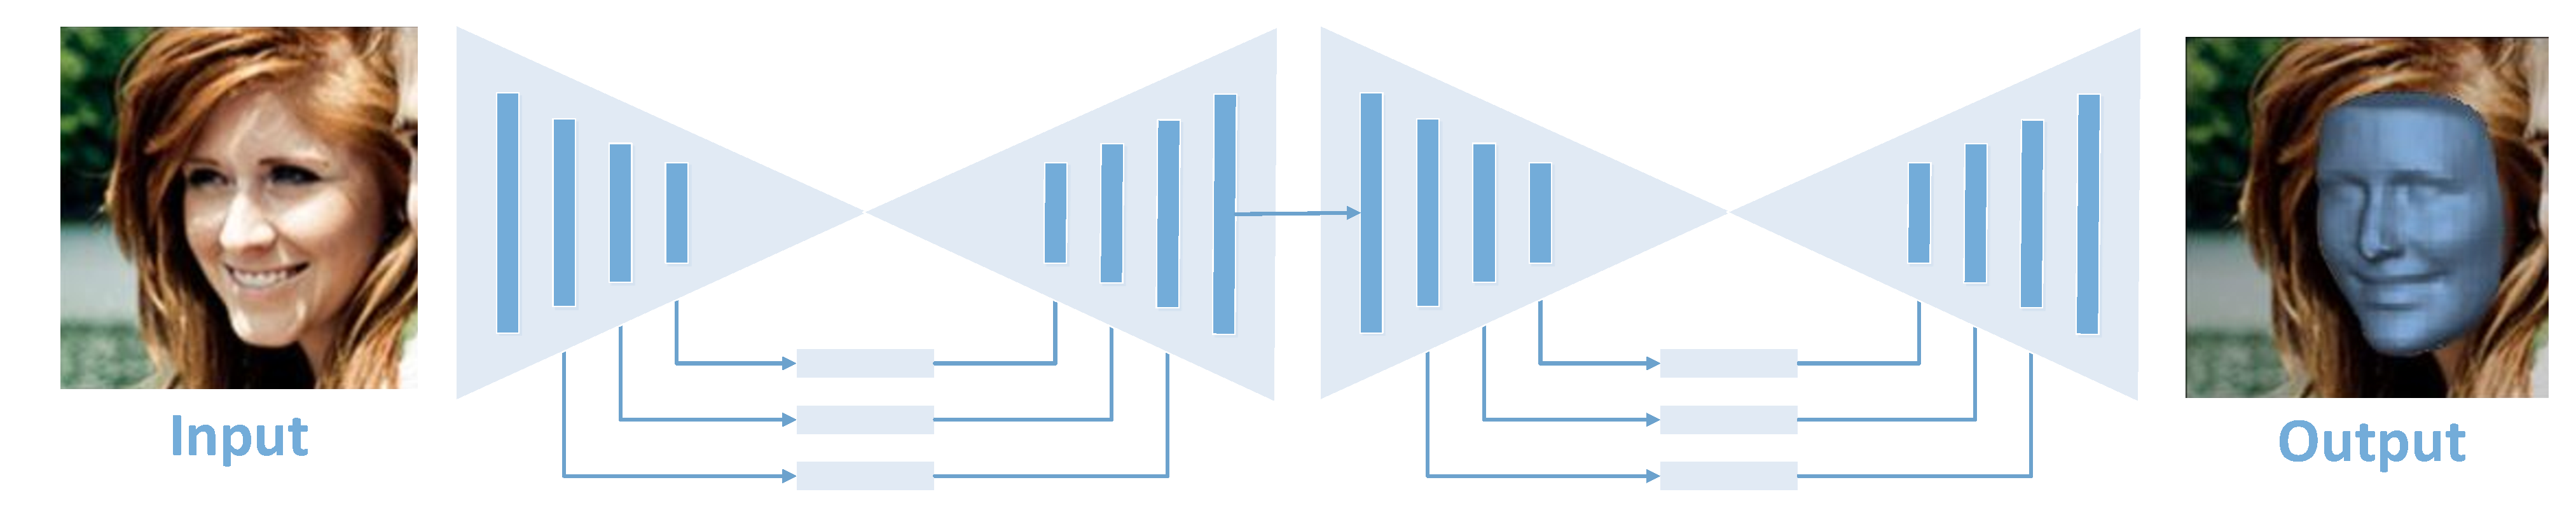
\includegraphics[width=0.81\linewidth]{img/baseline.pdf}
    \caption[Baseline reconstruction architecture]{The proposed
      \textit{Volumetric Regression Network (VRN)} accepts as input an
      RGB input and directly regresses a 3D volume completely bypassing
      the fitting of a 3DMM. Each rectangle is a residual module of 256
      features.}

    \label{fig:cnnbaseline}
  \end{subfigure}
  ~
  \begin{subfigure}[t]{0.98\textwidth}
    \centering
    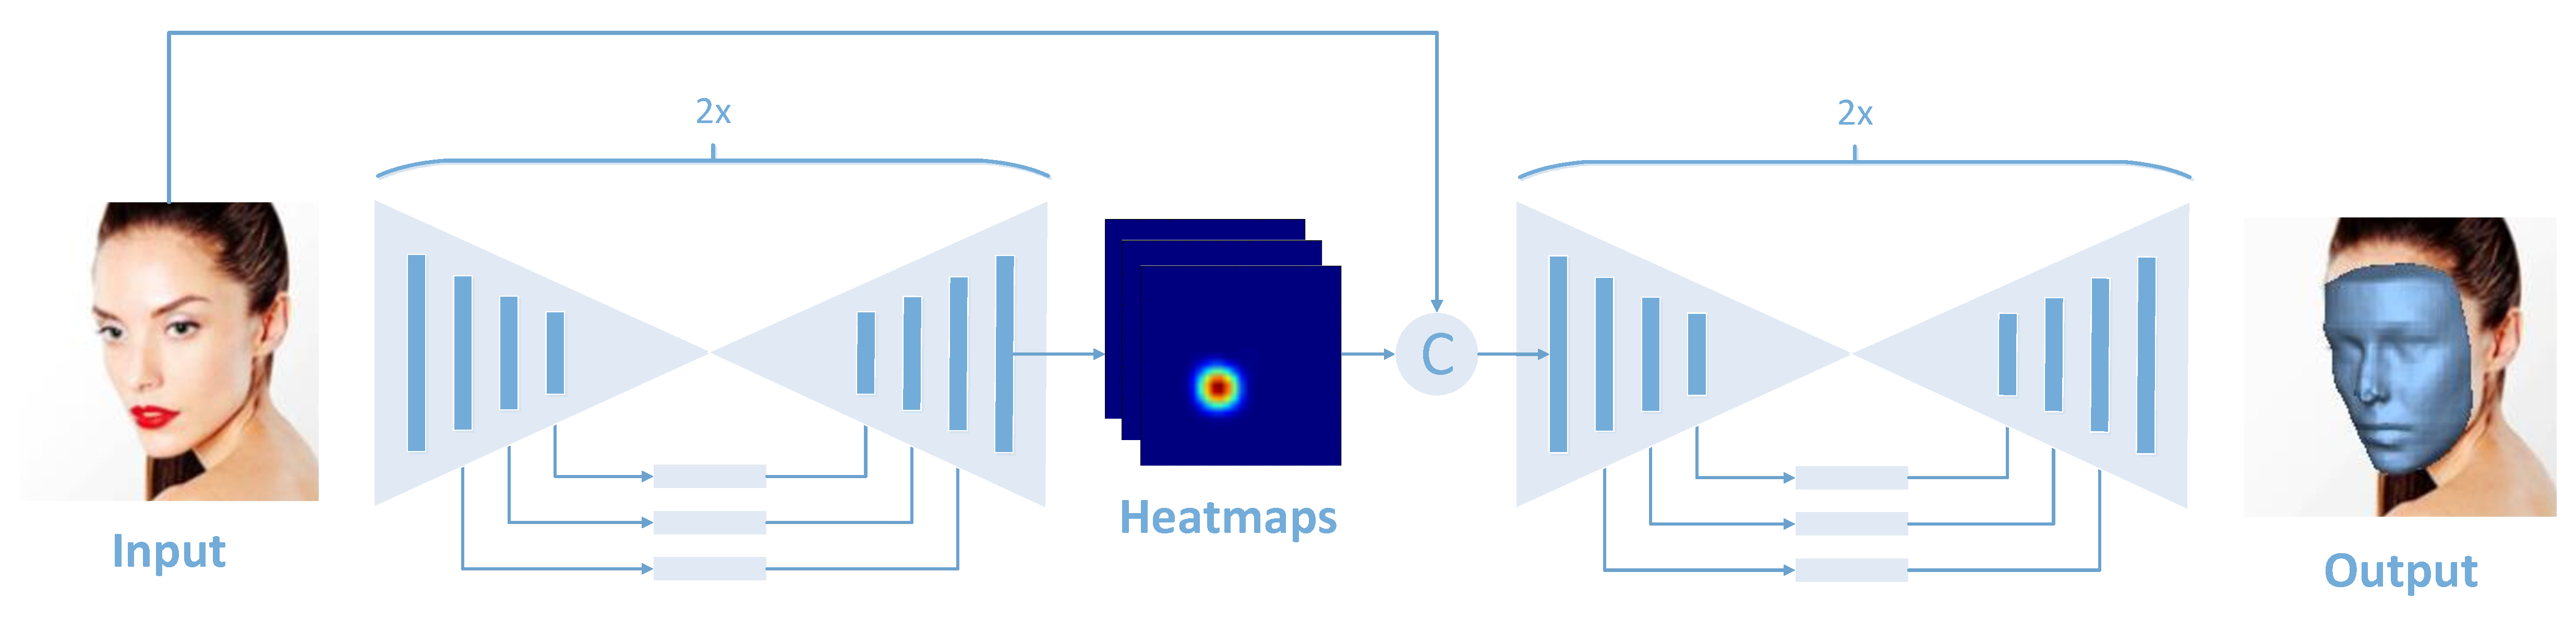
\includegraphics[width=\linewidth]{img/guided.pdf}
    \caption[Guided reconstruction architecture]{The proposed
      \textit{VRN - Guided} architecture firsts detects the 2D
      projection of the 3D landmarks, and stacks these with the original
      image. This stack is fed into the reconstruction network, which
      directly regresses the volume.}
    \label{fig:guidednet}
  \end{subfigure}
  ~
  \begin{subfigure}[t]{1\textwidth}
    \centering
    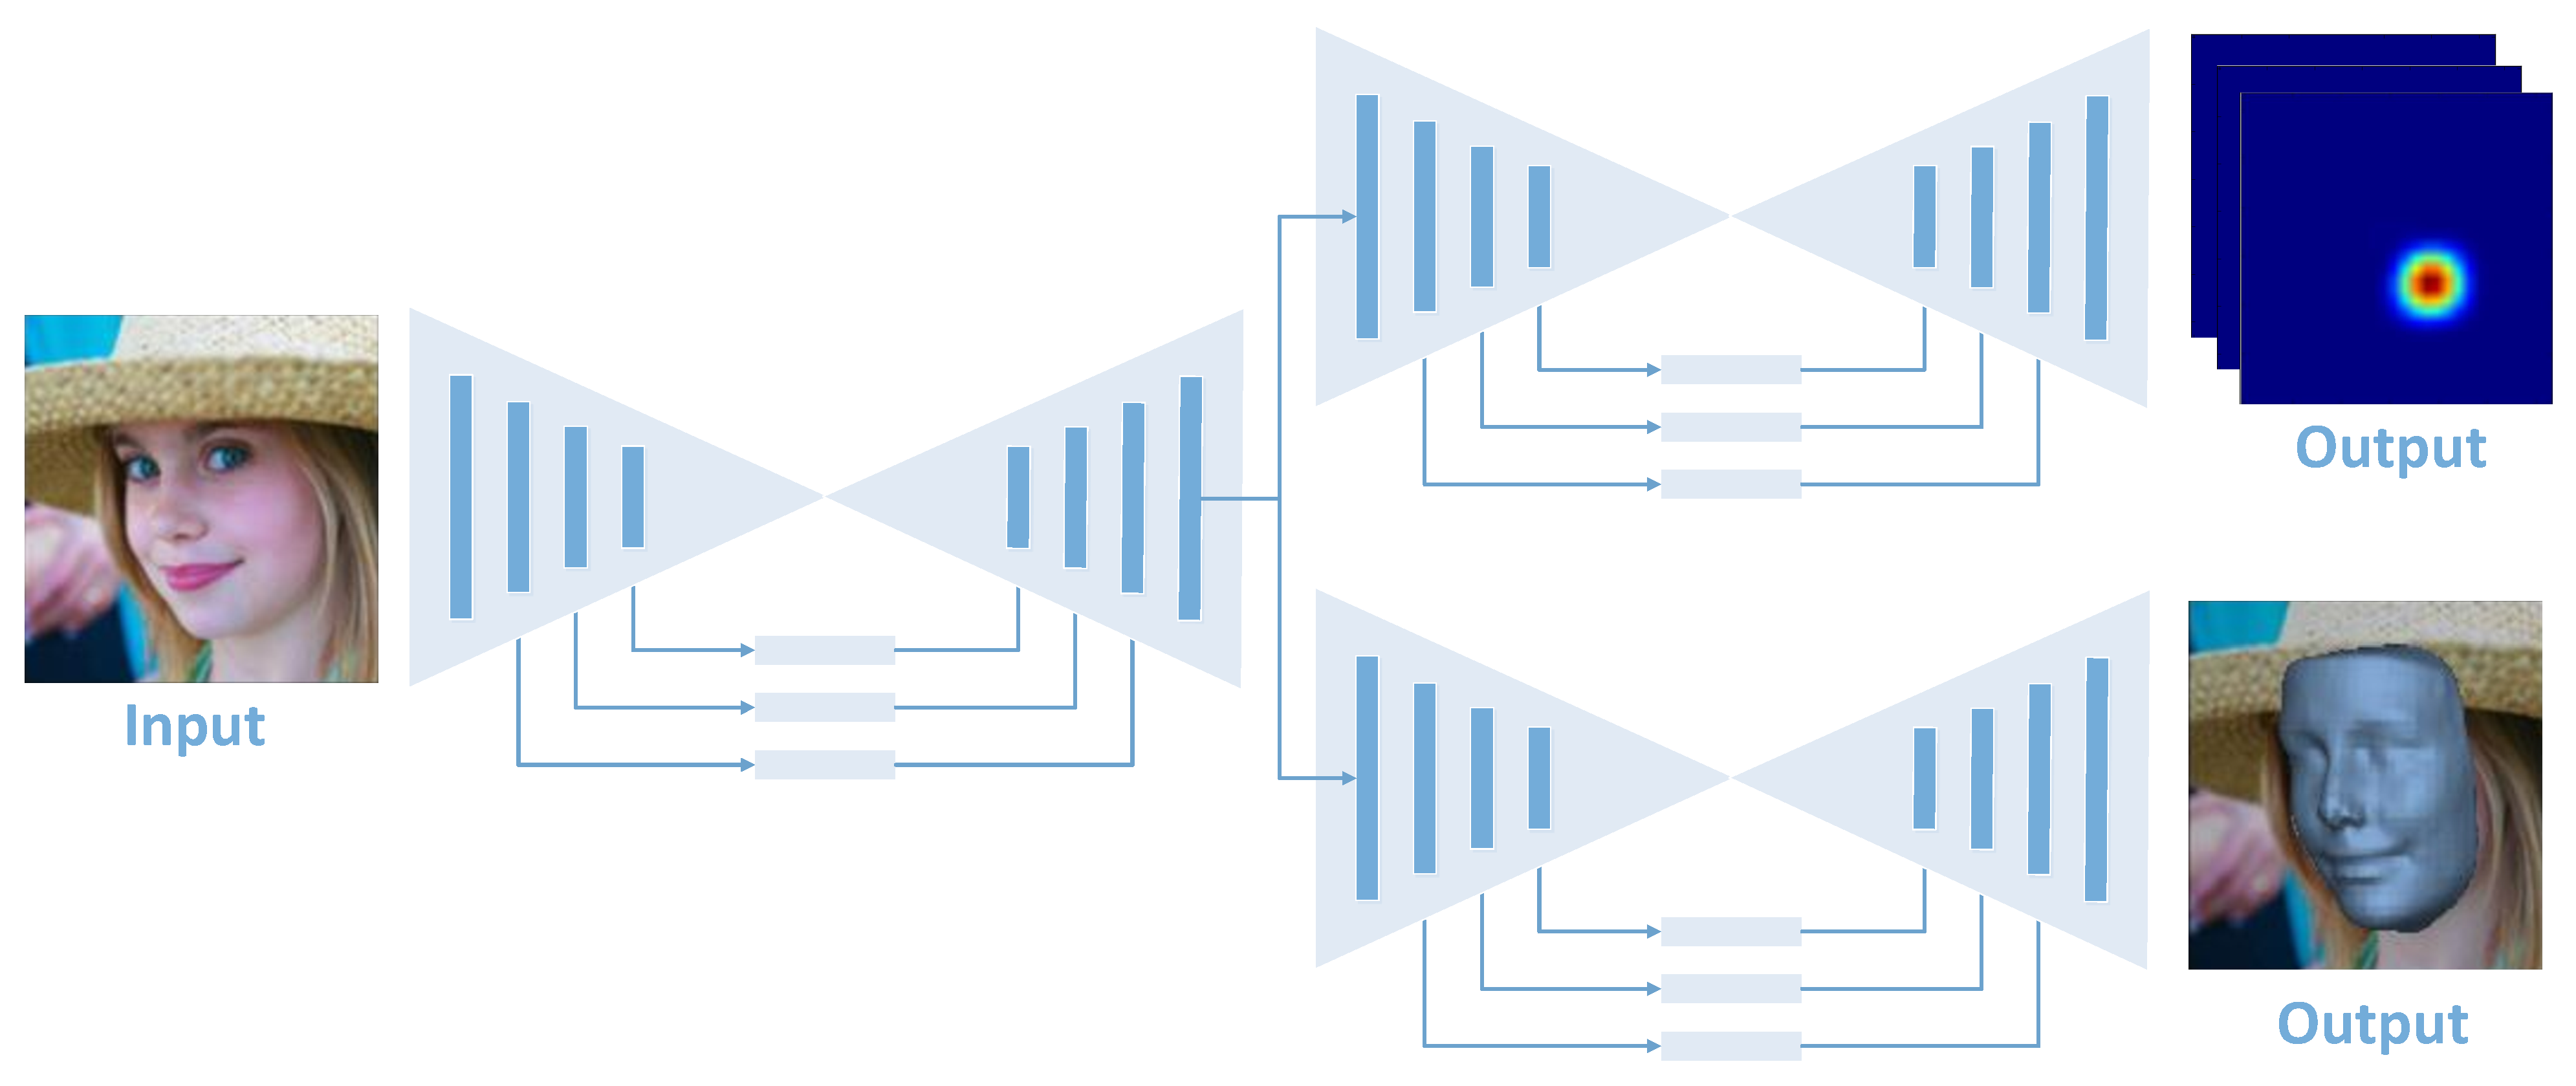
\includegraphics[width=0.6\linewidth]{img/multitask.pdf}
    \caption[Multitask reconstruction architecture]{The proposed
      \textit{VRN - Multitask} architecture regresses both the 3D facial
      volume and a set of sparse facial landmarks.}
    \label{fig:cnnmultitask}
    \vspace{-2mm}
  \end{subfigure}
  \caption[Overview of proposed architectures]{An overview of the
    proposed three architectures for Volumetric Regression:
    \textit{Volumetric Regression Network (VRN)}, \textit{VRN -
      Guided} and \textit{VRN - Multitask}.}
  \label{fig:cnnall}
  \vspace{-5mm}
\end{figure*}

We train our volumetric regression network using the sigmoid cross
entropy loss function:
\begin{equation} l_{1} = \sum\limits_{w=1}^{W}
  \sum\limits_{h=1}^{H}\sum\limits_{d=1}^{D}[V_{whd}\log
  \widehat{V}_{whd}+(1-V_{whd})\log(1-\widehat{V}_{whd})],
\end{equation} where $\widehat{V}_{whd}$ is the corresponding Sigmoid
output at voxel $\{w,h,d\}$ of the regressed volume.

At test time, and given an input 2D image, the network regresses a 3D
volume from which the outer 3D facial mesh is recovered. Rather than
making hard (binary) predictions at pixel level, we found that the
soft sigmoid output is more useful for further processing. Both
representations are shown in Figure~\ref{fig:roughvssmooth} where
clearly the latter results in smoother results. Finally, from the 3D
volume, a mesh can be formed by generating the iso-surface of the
volume. If needed, correspondence between this variable length mesh
and a fixed mesh can be found using Iterative Closest Point (ICP).

\textbf{VRN - Multitask}. We also propose a Multitask VRN, shown in
Figure~\ref{fig:cnnmultitask}, consisting of three hourglass
modules. The first hourglass provides features to a fork of two
hourglasses. The first of this fork regresses the 68 iBUG landmarks
\cite{sagonas2013semi} as 2D Gaussians, each on a separate
channel. The second hourglass of this fork directly regresses the 3D
structure of the face as a volume, as in the aforementioned unguided
volumetric regression method. The goal of this multitask network is to
learn more reliable features which are better suited to the two tasks.


\begin{figure}
  \centering
  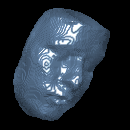
\includegraphics[width=0.2\linewidth]{img/example_rough.png}
  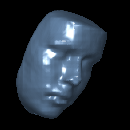
\includegraphics[width=0.2\linewidth]{img/example_smooth.png}
  \caption[Binary vs Real volumes]{Comparison between making hard
    (binary) vs soft (real) predictions. The latter produces a
    smoother result.}
  \label{fig:roughvssmooth}
  \vspace{-4mm}
\end{figure}


\textbf{VRN - Guided}. We argue that reconstruction should benefit
from firstly performing a simpler face analysis task; in particular we
propose an architecture for volumetric regression guided by facial
landmarks. To this end, we train a stacked hourglass network which
accepts guidance from landmarks during training and inference. This
network has a similar architecture to the unguided volumetric
regression method, however the input to this architecture is an RGB
image stacked with 68 channels, each containing a Gaussian ($\sigma =
1$, approximate diameter of 6 pixels) centred on each of the 68
landmarks. This stacked representation and architecture is
demonstrated in Figure~\ref{fig:guidednet}. During training we used the
ground truth landmarks while during testing we used a stacked
hourglass network trained for facial landmark localisation. We call
this network \textit{VRN - Guided}.




\subsection{Training}

% Trained with RMSProp
Each of our architectures was trained end-to-end using RMSProp with an
initial learning rate of $10^{-4}$, which was lowered after 40 epochs
to $10^{-5}$. During training, random augmentation was applied to each
input sample (face image) and its corresponding target (3D volume): we
applied in-plane rotation $r\in[-45^{\circ}, ..., 45^{\circ}]$,
translation $t_z,t_y\in[-15,...,15]$ and scale $s\in [0.85,...,1.15]$
jitter. In 20\% of cases, the input and target were flipped
horizontally. Finally, the input samples were adjusted with some
colour scaling on each RGB channel. % selected uniformly
$c_r,c_g,c_b \in \{0.6,...,1.4\}$.

In the case of the \textit{VRN - Guided}, the landmark detection
module was trained to regress Gaussians with standard deviation of
approximately 3 pixels ($\sigma = 1$). %We noticed near negligible
reduction in 3D reconstruction performance when training with
different standard deviations.

% dataset selection

% Gaussian size (sigma 1)
% Learning rate

\section{Results} \label{S:Results}

\begin{figure}
  \centering
  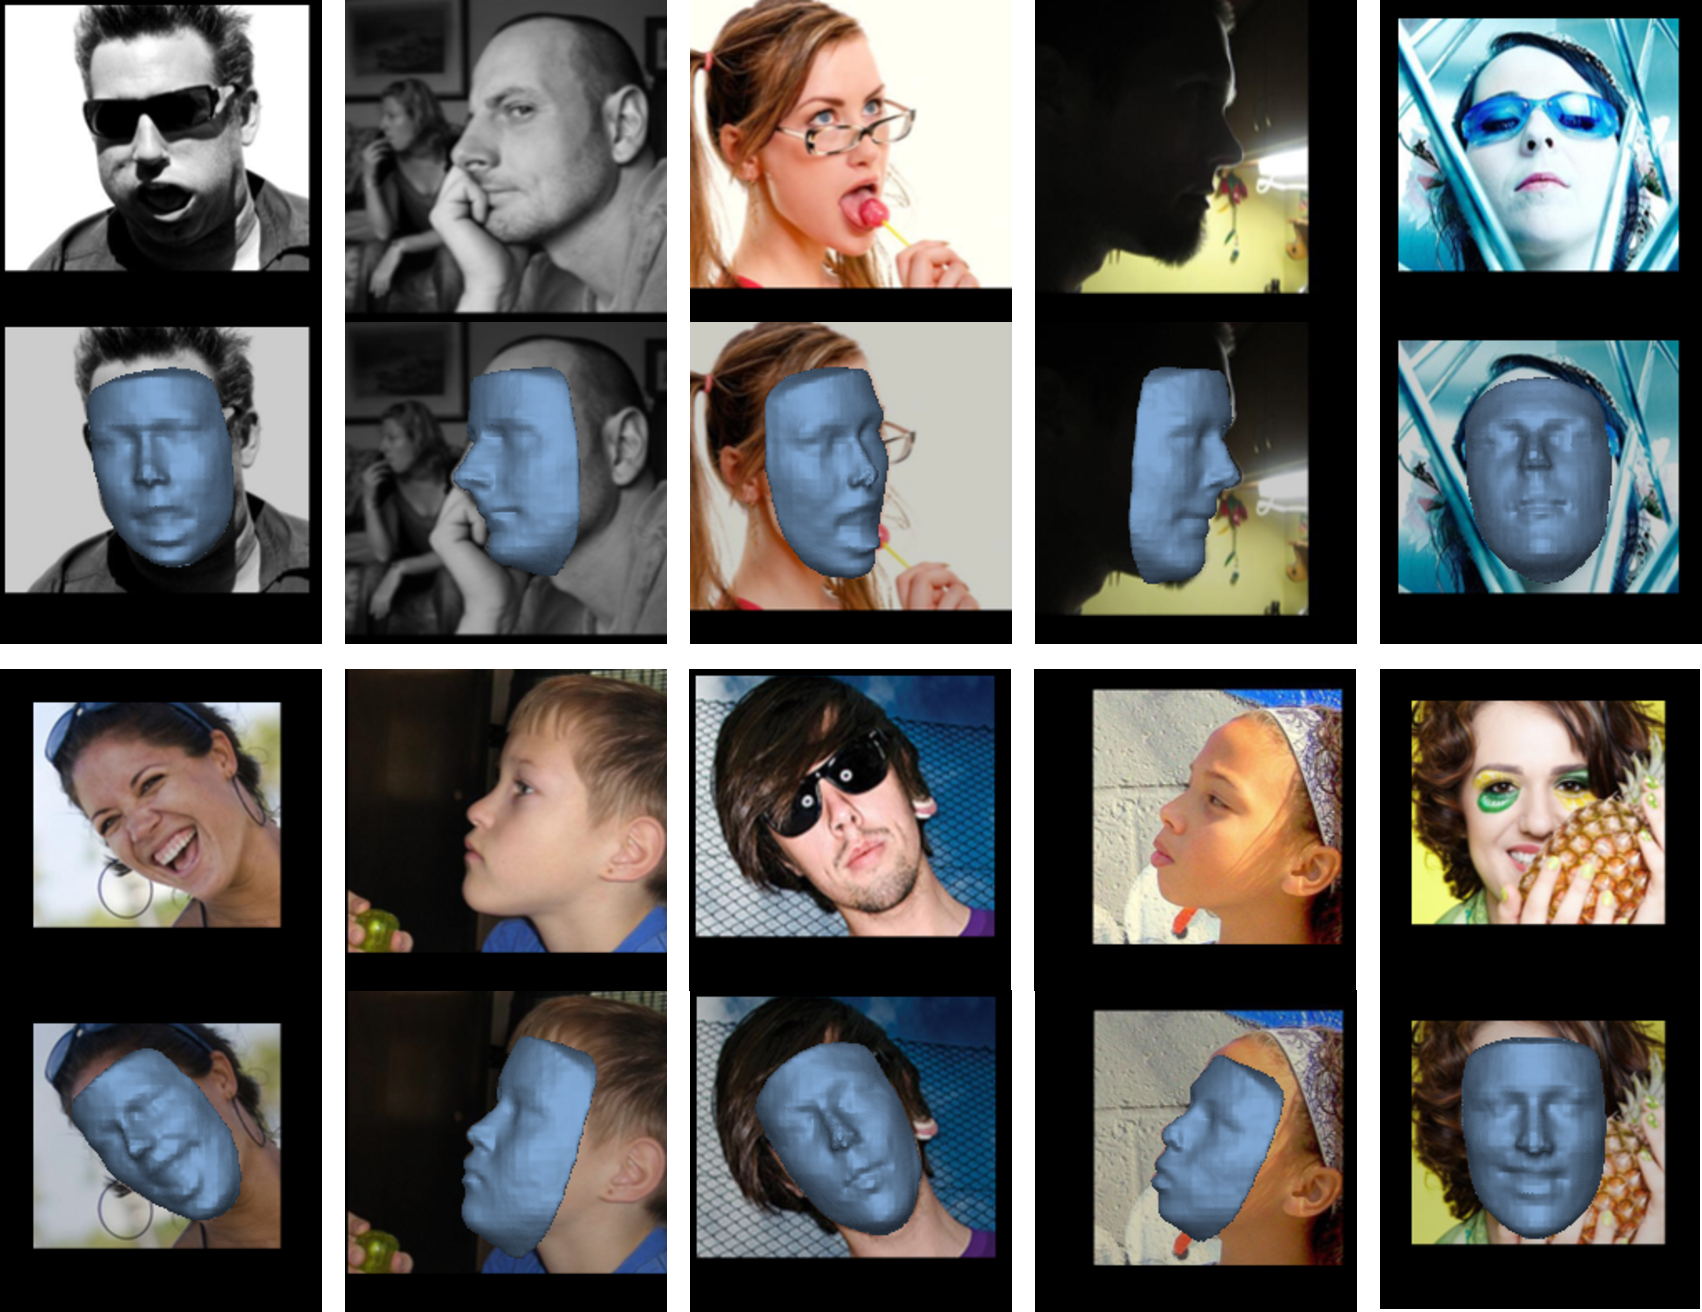
\includegraphics[width=0.7\linewidth]{img/aflw2000res.pdf}
  \caption[Visual results on AFLW2000-3D dataset]{Some visual results
    from the AFLW2000-3D dataset generated using our \textit{VRN -
      Guided} method.}
  \label{fig:aflw2000res}
  \vspace{-4mm}
\end{figure}

\begin{figure}
  \centering
  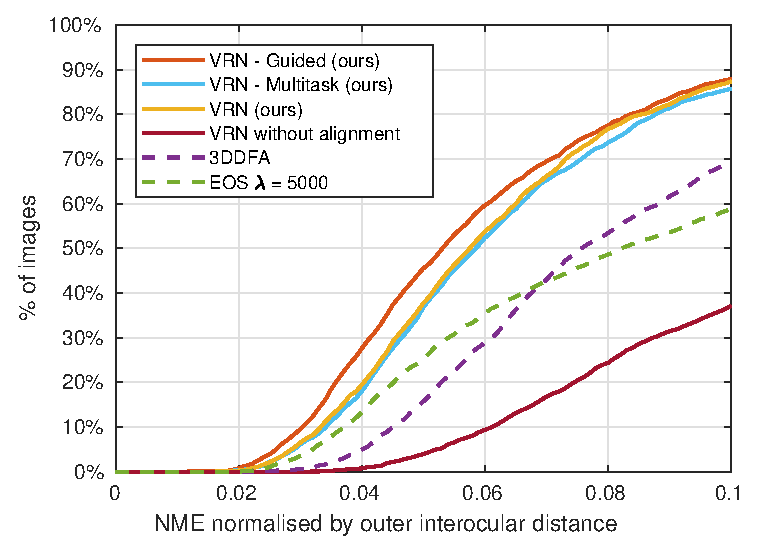
\includegraphics[width=0.75\linewidth]{curves/aflw.eps}
  \caption[NME performance on AFLW2000-3D images]{NME-based
    performance on in-the-wild ALFW2000-3D dataset. The proposed
    \textit{Volumetric Regression Networks}, and EOS and 3DDFA are
    compared.}
  \label{roc:aflw2000}
\end{figure}

\begin{figure}
  \centering
  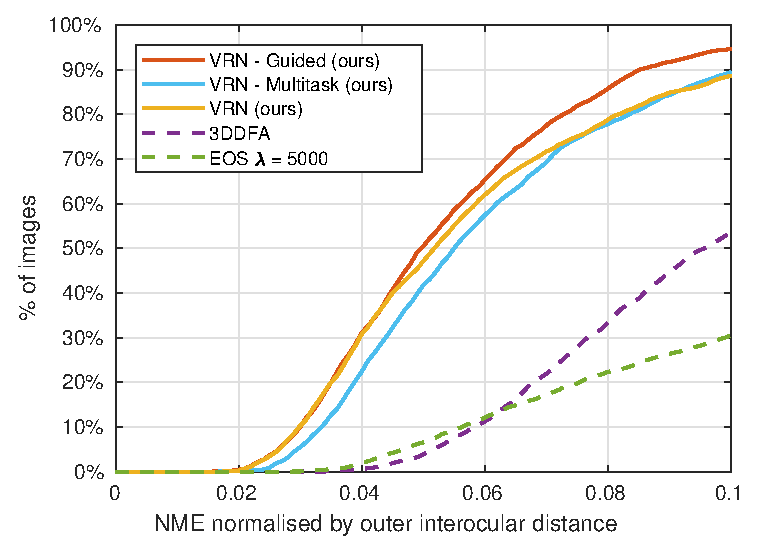
\includegraphics[width=0.75\linewidth]{curves/bu4dfe.eps}
  \caption[NME performance on BU-4DFE renderings]{NME-based
    performance on renderings from BU-4DFE. The proposed
    \textit{Volumetric Regression Networks}, and EOS and 3DDFA are
    compared.}
  \label{roc:bu4dfe}
\end{figure}

\begin{figure}
  \centering
  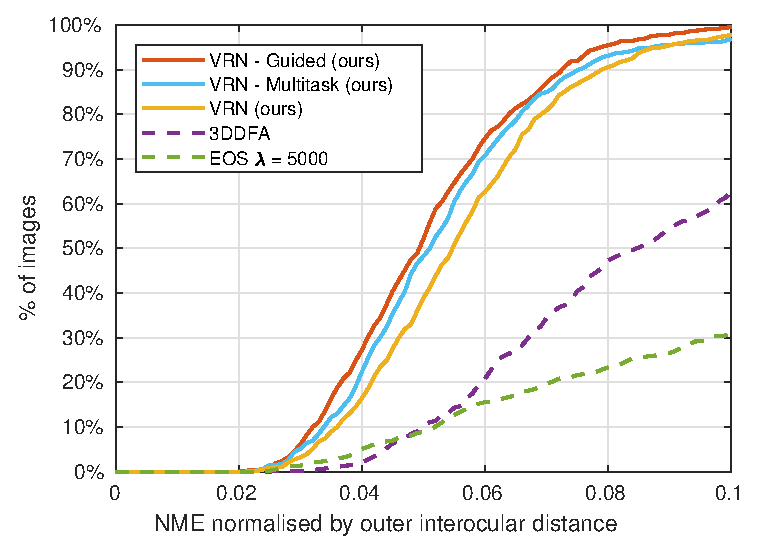
\includegraphics[width=0.75\linewidth]{curves/florence.eps}
  \caption[NME performance on Florence renderings]{NME-based
    performance on our large pose renderings of the Florence
    dataset. The proposed \textit{Volumetric Regression Networks}, and
    EOS and 3DDFA are compared.}
  \label{roc:florence}
\end{figure}



\begin{table}
  \caption[Numerical performance of 3D face
  reconstruction]{Reconstruction accuracy on AFLW2000-3D, BU-4DFE and
    Florence in terms of NME. Lower is better.}
  \label{tab:overview}
  \centering
  \small
  \begin{tabular}{|l||c|c|c|}
    \hline
    \textbf{Method}   & \textbf{AFLW2000-3D} & \textbf{BU-4DFE} & \textbf{Florence} \\
    \hline\hline
    VRN & 0.0676   & 0.0600 & 0.0568   \\
    VRN - Multitask   & 0.0698        & 0.0625     & 0.0542        \\
    VRN - Guided    & \textbf{0.0637}   & \textbf{0.0555} & \textbf{0.0509}   \\
    \hline
    3DDFA~\cite{zhu2016face}             & 0.1012   & 0.1227 & 0.0975   \\
    EOS~\cite{huber2016multiresolution}  & 0.0971   & 0.1560 & 0.1253   \\
    \hline
  \end{tabular}
  \vspace{-4mm}
\end{table}


We performed cross-database experiments only, on 3 different
databases, namely AFLW2000-3D, BU-4DFE, and Florence reporting the
performance of all the proposed networks (\textit{VRN}, \textit{VRN -
  Multitask} and \textit{VRN - Guided}) along with the performance of
two state-of-the-art methods, namely 3DDFA \cite{zhu2016face} and EOS
\cite{huber2016multiresolution}. Both methods perform 3DMM
fitting (3DDFA uses a CNN), a process completely bypassed by \textit{VRN}.


Our results can be found in Table~\ref{tab:overview} and
Figures~\ref{roc:aflw2000},~\ref{roc:bu4dfe} and~\ref{roc:florence}.
Visual results of the proposed \textit{VRN - Guided} on some very
challenging images from AFLW2000-3D can be seen in
Figure~\ref{fig:aflw2000res}. Examples of failure cases along with a
visual comparison between \textit{VRN} and \textit{VRN - Guided} can
be found in the supplementary material. From these results, we can
conclude the following:
\begin{enumerate}
\item Volumetric Regression Networks largely outperform 3DDFA and EOS
  on all datasets, verifying that directly regressing the 3D facial
  structure is a much easier problem for CNN learning.
\item All VRNs perform well across the whole spectrum of facial poses,
  expressions and occlusions. Also, there are no significant performance
  discrepancies across different datasets (ALFW2000-3D seems to be
  slightly more difficult).
\item The best performing VRN is the one guided by detected landmarks
  (\textit{VRN - Guided}), however at the cost of higher computational
  complexity: \textit{VRN - Guided} uses another stacked hourglass
  network for landmark localization.
\item \textit{VRN - Multitask} does not always perform particularly
  better than the plain VRN (in fact on BU-4DFE it performs worse), not
  justifying the increase of network complexity. It seems that it might
  be preferable to train a network to focus on the task in hand.
\end{enumerate}

\noindent Details about our experiments are given in the proceeding subsections.

\subsection{Datasets}

We used three different datasets for quantifying the performance of
our method. The dataset AFLW2000-3D allows for unbiased and fair
comparison with other methods. The remaining two, BU-4DFE and
Florence, have to be rendered, but allows us to quantify performance
across pose and expression with greater accuracy. These three datasets
are discussed in more detail below.

\paragraph{(a) AFLW2000-3D} As our target was to test
our network on totally unconstrained images, we firstly conducted
experiments on the AFLW2000-3D~\cite{zhu2016face} dataset which
contains 3D facial meshes for the first 2000 images from AFLW
\cite{aflw2011}.

\paragraph{(b) BU-4DFE} We also conducted experiments
on rendered images from BU-4DFE~\cite{yin2008high}. We rendered each
participant for both Happy and Surprised expressions with three
different pitch rotations between $-20$ and $20$ degrees. For each
pitch, seven roll rotations from $-80$ to $80$ degrees were also
rendered. Large variations in lighting direction and colour were added
randomly to make the images more challenging.

\paragraph{(c) Florence}
Finally, we conducted experiments on rendered images from the
Florence~\cite{masi2d3dFaceData} dataset. Facial images were rendered
in a similar fashion to the ones of BU-4DFE but for slightly different
parameters: Each face is rendered in 20 difference poses, using a
pitch of -15, 20 or 25 degrees and each of the five evenly spaced
rotations between -80 and 80.

\subsubsection{Error metric} To measure the accuracy of reconstruction for
each face, we used the Normalised Mean Error (NME) defined as the
average per vertex Euclidean distance between the estimated and ground
truth reconstruction normalised by the outer 3D interocular distance:

\begin{equation}
  \textrm{NME} = \frac{1}{N} \sum_{k=1}^{N} \frac{||\mathbf{x}_k-\mathbf{y}_{k} ||_{2} }{d}, \label{eq:err}
\end{equation}
where $N$ is the number of vertices per facial mesh, $d$ is the 3D
interocular distance and $\mathbf{x}_k$,$\mathbf{y}_k$ are vertices of
the grouthtruth and predicted meshes. The error is calculated on the
face region only on approximately 19,000 vertices per facial
mesh. Notice that when there is no point correspondence between the
ground truth and the estimated mesh, ICP was used but only to
establish the correspondence, i.e. the rigid alignment was not
used. If the rigid alignment is used, we found that, for all methods,
the error decreases but it turns out that the relative difference in
performance remains the same. For completeness, we included these
results in the supplementary material.

\subsubsection{Comparison with state-of-the-art}
We compared against state-of-the-art 3D reconstruction methods for
which code is publicly available. These include the very recent
methods of 3DDFA~\cite{zhu2016face}, and
EOS~\cite{huber2016multiresolution}. For EOS we used a large
regularisation parameter $\lambda = 5000$ which we found to offer the
best performance for most images. The method uses 2D landmarks as
input, so for the sake of a fair comparison a stacked hourglass for 2D
landmark detection was trained for this purpose. Our tests were
performed using v0.12 of EOS.


\section{Importance of spatial alignment}
\label{sec:spatialimportance}

The 3D reconstruction method described in~\cite{choy20163d} regresses
a 3D volume of fixed orientation from one or more images using an
LSTM. This is different to our approach of taking a single image and
regressing a spatially aligned volume, which we believe is easier to
learn. To explore what the repercussions of ignoring spatial alignment
are, we trained a variant of \textit{VRN} which regresses a frontal
version of the face, i.e. a face of fixed orientation as in
~\cite{choy20163d}. We also attempted to train a network using the
code from~\cite{choy20163d} on downsampled versions of our own
volumes. Unfortunately, we were unable to get the network to learn
anything.

Although this network produces a reasonable face, it can only capture
diminished expression, and the shape for all faces appears to remain
almost identical. This is very noticeable in
Figure~\ref{fig:frontal_visual}. Numeric comparison is shown in
Figure~\ref{roc:aflw2000}, as \textit{VRN without alignment}. We
believe that this further confirms that spatial alignment is of
paramount importance when performing 3D reconstruction in this way.

\begin{figure}
  \centering
  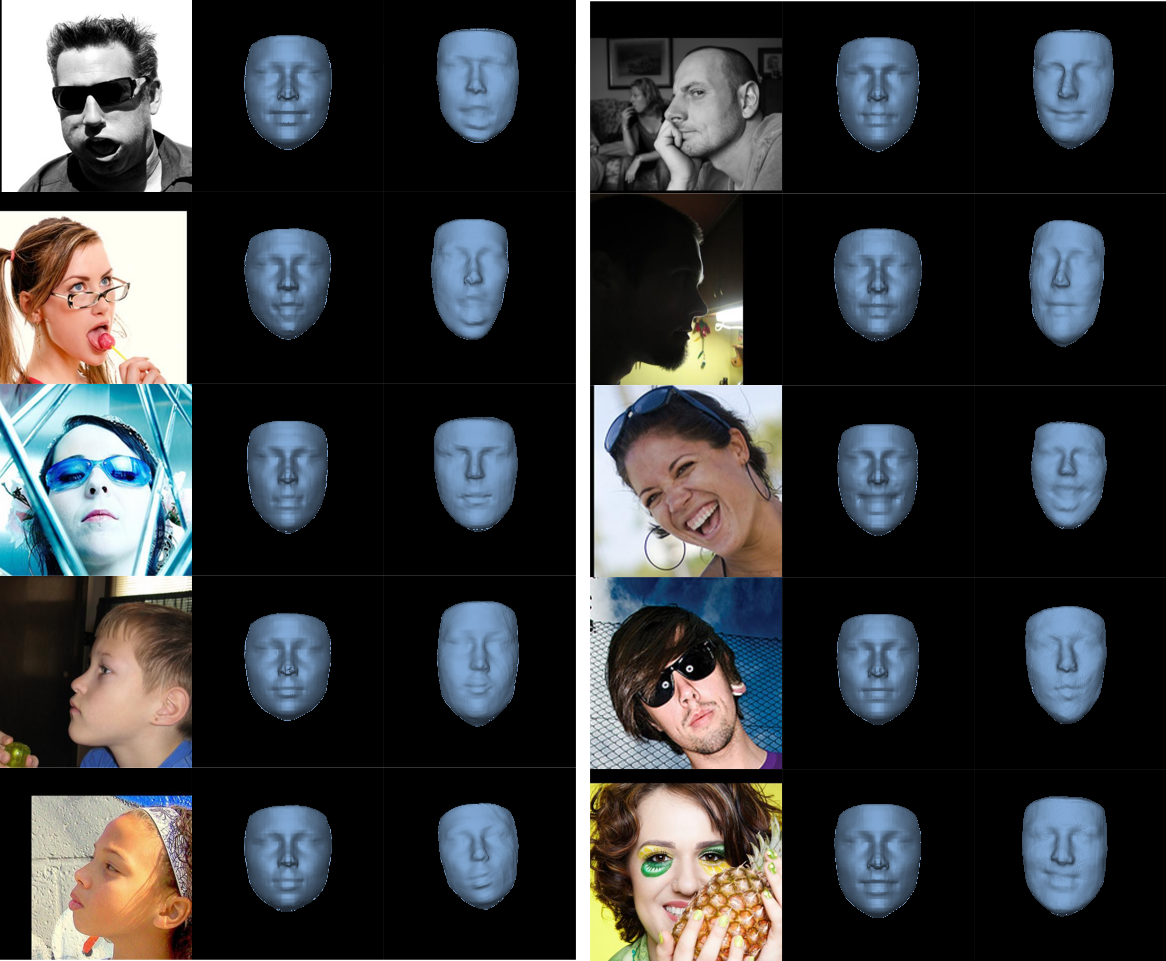
\includegraphics[width=0.7\linewidth]{img/frontal.png}
  \caption[Visual results when spatial alignment is ignored]{Result from
    \textit{VRN without alignment} (second columns), and a frontalised
    output from \textit{VRN - Guided} (third columns).}
  \label{fig:frontal_visual}
\end{figure}

\section{Ablation studies}
\label{chapter:face:sec:ablation}

In this section, we report the results of experiments aiming to shed
further light into the performance of the proposed networks. For all
experiments reported, we used the best performing \textit{VRN -
  Guided}.

\subsection{Effect of pose}
To measure the influence of pose on the reconstruction error, we
measured the NME for different yaw angles using all of our
Florence~\cite{masi2d3dFaceData} renderings. As shown in
Figure~\ref{fig:effect_pose}, the performance of our method decreases as
the pose increases. This is to be expected, due to less of the face
being visible which makes evaluation for the invisible part
difficult. We believe that our error is still very low considering
these poses.


\subsection{Effect of expression} Certain expressions are usually
considered harder to accurately reproduce in 3D face
reconstruction. To measure the effect of facial expressions on
performance, we rendered frontal images in difference expressions from
BU-4DFE (since Florence only exhibits a neutral expression) and
measured the performance for each expression. This kind of extreme
acted facial expressions generally do not occur in the training set,
yet as shown in Figure~\ref{fig:effect_expression}, the performance
variation across different expressions is quite minor.

\begin{figure}
  \centering
  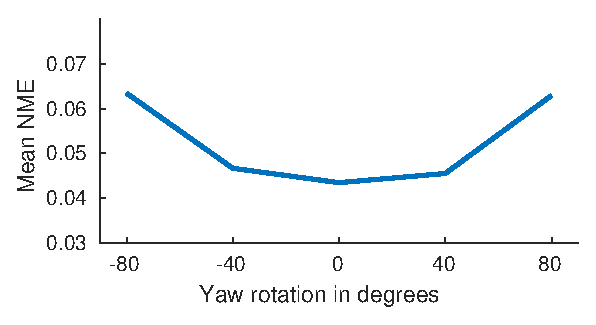
\includegraphics[width=0.5\linewidth]{curves/ablation_pose.eps}
  \caption[Effect of pose]{The effect of pose on reconstruction
    accuracy in terms of NME on the Florence dataset. The \textit{VRN
      - Guided} network was used.}
  \label{fig:effect_pose}
\end{figure}


\begin{figure}
  \centering
  
\includegraphics[width=0.7\linewidth]{curves/ablation_expression.eps}
  \caption[Effect of facial expressions]{The effect of facial
    expression on reconstruction accuracy in terms of NME on the
    BU-4DFE dataset. The \textit{VRN - Guided} network was used.}
  \label{fig:effect_expression}
\end{figure}

\subsection{Effect of Gaussian size for guidance} We trained a
\textit{VRN - Guided}, however, this time, the facial landmark
detector network of the \textit{VRN - Guided} regresses larger
Gaussians ($\sigma = 2$ as opposed to the normal $\sigma = 1$). The
performance of the 3D reconstruction dropped by a negligible amount,
suggesting that as long as the Gaussians are of a sensible size,
guidance will always help.



\section{Conclusions}

We proposed a direct approach to 3D facial reconstruction from a
single 2D image using volumetric CNN regression. To this end, we
proposed and exhaustively evaluated three different networks for
volumetric regression, reporting results that show that the proposed
networks perform well for the whole spectrum of facial pose, and can
deal with facial expressions as well as occlusions. We also compared
the performance of our networks against that of recent
state-of-the-art methods based on 3DMM fitting reporting large
performance improvement on three different datasets.  Future work may
include improving detail and establishing a fixed correspondence from
the isosurface of the mesh.


%%% Local Variables:
%%% TeX-master: "../thesis"
%%% End: